\documentclass[a4paper,12pt]{article}

%%% Работа с русским языком

\usepackage{cmap}					% поиск в PDF
\usepackage{mathtext} 				% русские буквы в формулах
\usepackage[T2A]{fontenc}			% кодировка
\usepackage[utf8]{inputenc}			% кодировка исходного текста
\usepackage[english,russian]{babel}	% локализация и переносы
\usepackage{indentfirst}            % красная строка в первом абзаце
\usepackage[unicode]{hyperref}
\usepackage{epigraph}
% \usepackage{algorithm}     % algo
% \usepackage{algpseudocode} % algo
\usepackage{algorithm2e}
\frenchspacing                      % равные пробелы между словами и предложениями

%%% Дополнительная работа с математикой
\usepackage{amsmath,amsfonts,amssymb,amsthm,mathtools} % пакеты AMS
\usepackage{bbm} % Blackboard bold для цифр
\usepackage{icomma}                                    % "Умная" запятая

\renewcommand{\phi}{\ensuremath{\varphi}}
\renewcommand{\kappa}{\ensuremath{\varkappa}}
\renewcommand{\le}{\ensuremath{\leqslant}}
\renewcommand{\leq}{\ensuremath{\leqslant}}
\renewcommand{\ge}{\ensuremath{\geqslant}}
\renewcommand{\geq}{\ensuremath{\geqslant}}
\renewcommand{\emptyset}{\ensuremath{\varnothing}}

\newcommand{\cl}{\text{cl }}
\newcommand{\setint}{\text{int }}



\theoremstyle{plain}
\newtheorem{theorem}{Теорема}[section]
\newtheorem{lemma}{Лемма}[section]
\newtheorem{proposition}{Утверждение}[section]
\newtheorem*{corollary}{Следствие}
\newtheorem*{exercise}{Упражнение}

\theoremstyle{definition}
\newtheorem{definition}{Определение}[section]
\newtheorem*{note}{Замечание}
\newtheorem*{reminder}{Напоминание}
\newtheorem*{example}{Пример}
\newtheorem*{tasks}{Задача}

\theoremstyle{remark}
\newtheorem*{solution}{Решение}

%%% Оформление страницы
\usepackage{extsizes}     % Возможность сделать 14-й шрифт
\usepackage{geometry}     % Простой способ задавать поля
\usepackage{setspace}     % Интерлиньяж
\usepackage{enumitem}     % Настройка окружений itemize и enumerate
\setlist{leftmargin=25pt} % Отступы в itemize и enumerate

\geometry{top=25mm}    % Поля сверху страницы
\geometry{bottom=30mm} % Поля снизу страницы
\geometry{left=20mm}   % Поля слева страницы
\geometry{right=20mm}  % Поля справа страницы

\newcommand{\coursedate}{Весна 2023}
\date{Весна 2023}

\title{
    <<Метрическая задача коммивояжёра>>  \\ 
    \large ФПМИ МФТИ }
\newcommand{\coursename}{Сложности вычислений, 4 семестр}

\author{
    {Тимур Зыков, Б05-121} % Тут можно вставить ссылку на свой вк
    % \compiledby
}

\usepackage{titleps} 
\newpagestyle{main}{
  \setheadrule{.4pt}                      
  \sethead{\coursename}{}{\hyperlink{intro}{\;Назад к содержанию}}
  \setfootrule{.4pt}                       
  \setfoot{\coursedate \; ФПМИ МФТИ}{}{\thepage} 
}     

\pagestyle{main}

\begin{document}
\maketitle

\newpage
\begin{abstract}
    Задача коммивояжёра (или TSP от англ. travelling salesman problem) — одна из самых известных задач комбинаторной оптимизации, заключающаяся в поиске самого выгодного маршрута, проходящего через указанные города хотя бы по одному разу с последующим возвратом в исходный город. Вместе с простотой определения и сравнительной простотой нахождения хороших решений задача коммивояжёра отличается тем, что нахождение действительно оптимального пути является достаточно сложной задачей. Учитывая эти свойства, начиная со второй половины XX века исследование задачи коммивояжёра имеет не столько практический смысл, сколько теоретический в качестве модели для разработки новых алгоритмов оптимизации.
\end{abstract}
  
\tableofcontents

\newpage

\section{Введение}
В 1950-е и 1960-е годы задача коммивояжёра привлекла внимание ученых в США и Европе. Важный вклад в исследование задачи принадлежит Джорджу Данцигу, Делберту Рею Фалкерсону и Селмеру Джонсону, которые в 1954 году в институте RAND Corporation сформулировали задачу в виде задачи дискретной оптимизации и применили для её решения метод отсечений. Используя этот метод, они построили путь коммивояжёра для одной частной постановки задачи с 49 городами и обосновали его оптимальность. В 1960-е и 1970-е годы задача изучалась многими учеными как теоретически, так и с точки зрения её приложений в информатике, экономике, химии и биологии.

Ричард Карп в 1972 году доказал NP-полноту задачи поиска гамильтоновых путей, из чего, благодаря полиномиальной сводимости, вытекала NP-трудность задачи коммивояжёра. На основе этих свойств им было приведено теоретическое обоснование сложности поиска решений задачи на практике.

Больших успехов удалось достичь в конце 1970-х и 1980-х годах, когда Мартин Грётчел, Манфред Падберг и Джованни Ринальди и другие, с применением новых методов деления плоскостью, ветвей и границ вычислили решение для отдельного случая задачи с 2393 городами.

В марте 2005 года задача с 33810 узлами была решена программой: был вычислен путь длиной в 66048945 и доказано отсутствие более коротких путей. В апреле 2006 было найдено решение для экземпляра с 85900 узлами.

На практике поиск строго оптимального маршрута требуется не всегда. Существуют алгоритмы поиска приближенных решений для метрической задачи за полиномиальное время и нахождения маршрута максимум вдвое длиннее оптимального.
\section{Основные понятия и утверждения}

\subsection{Определения и постановка задачи}
\begin{definition}
    Графом $G = \left(V, E\right)$ называется пара множества вершин и множества ребер.
\end{definition}

\begin{definition}
    Граф $K_n = \left(V, E\right)$, $\left|V\right| = n$ называется полным, если у него есть все возможные ребра. То есть $\left|E\right| = C_n^2$.
\end{definition}

\begin{definition}
    Маршрутом в графе $G = \left(V, E\right)$ будем называть чередующуюся последовательность вершин и ребер, которая начинается и заканчивается на вершинах.
    $$
        v_1e_1v_2\ldots e_nv_{n+1}, \forall e_i: e_i=\left(v_i, v_{i+1}\right)
    $$
\end{definition}

\begin{definition}
    Циклом назовем замкнутый маршрут, где все ребра разные.
\end{definition}

\begin{definition}
    Простой цикл это цикл, где все вершины разные.
\end{definition}

\begin{definition}
    Гамильтонов цикл - простой цикл, проходящий через все вершины по одному разу.
\end{definition}

\begin{definition}
    Классом \textbf{DTIME}$\left(T(n)\right)$ называется класс языков, которые распознаются за время $O(T(n))$.
\end{definition}

\begin{definition}
    $\textbf{P} = \bigcup_{i=1}^\infty \textbf{DTIME}\left(n^c\right)$
\end{definition}

\begin{definition}
    Классом \textbf{NTIME}$\left(T(n)\right)$ называется класс языков, которые распознаются на недетерминированной машине Тьюринга за время $O(T(n))$.
\end{definition}

\begin{definition}
    $\textbf{NP} = \bigcup_{i=1}^\infty \textbf{NTIME}\left(n^c\right)$
\end{definition}

\begin{note}
    $\textbf{P} \subset \textbf{NP}$
\end{note}

\begin{definition}
Язык $B$ является \textbf{NP}-трудным, если для любого $A \in$ \textbf{NP} выполнено $A \leq_p B$. Язык $B$ является \textbf{NP}-полным, если он \textbf{NP}-трудный и лежит в \textbf{NP}.
\end{definition}

\begin{note}
    Язык \textnormal{\textsf{HAMCYCLE}} $= \{ G$ $|$ в графе $G$ существует гамильтонов цикл$\}$ является \textbf{NP}-полным.
\end{note}

\begin{tasks}
    В общем случае задача коммивояжёра ставится так: дан граф $G = \left(V, E\right)$ и веса
    на рёбрах $w: E \rightarrow \mathbb{R}_+$. Требуется найти гамильтонов цикл минимального веса.
    В метрическом случае граф полный, а функция весов метрическая (то есть для
    любых трёх вершин $x$, $y$ и $z$ выполнено $w(x, z) \leq w(x, y) + w(y, z))$.
\end{tasks}

\begin{definition}
    Алгоритм дает $\alpha$-приближение, если он дает результат не более чем в $\alpha$ раз превосходяший истинный оптимальный.
\end{definition}

\begin{note}
    Можно рассматривать $\alpha = \alpha(n)$, где обычно $n = \left| V \right|$.
\end{note}


\subsection{NP-трудность}
В общем случае, задача коммивояжера не может быть приближена за полином, если \textbf{P} $\neq$ \textbf{NP}.

\begin{theorem}
    Для стандартной задачи коммивояжёра не существует константных алгоритмов приближения, работающих за полином и если \textbf{P} $\neq$ \textbf{NP}.
\end{theorem}

\begin{proof}
    Сведем задачу \textsf{HAMCYCLE} к поиску $\alpha$-приближения в задаче коммивояжёра. Пусть дан граф $G = \left(V, E\right)$. Сделаем его полным $G' = \left(V, E'\right)$, где рёбра из $E$ имеют вес 1, другие имеют вес $K > \alpha n$. Тогда, если в исходном графе был гамильтонов цикл, в новом графе будет цикл коммивояжера длины $n$. Иначе в любом цикле будет ребро не из $E$ --- не было гамильтонова цикла изначалально.
\end{proof}

\section{Алгоритмы приближений метрической задачи коммивояжёра}
Если мы ограничимся графами, функции веса ребёр которых удовлетворяет неравенству треугольника, т.е. рассмотрим метрическую задачу коммивояжёра, задача остается NP-трудной, но ее уже не трудно 
аппроксимировать. Для таких задач построены полиномиальные приближённые алгоритмы, так называемые \textsf{PTAS} (polynomial-time approximation schemes — аппроксисмирующие схемы, работающие за полиномиальное время). 

\begin{definition}
    Деревом называется связный ацикличный граф.
\end{definition}

\begin{definition}
    Минимальное остовное дерево (\textsf{MST}) -- подграф-дерево минимального веса, которое содержит все исходные вершины.
\end{definition}

\begin{definition}
    Эйлеров цикл -- цикл, проходящий через каждое ребро графа ровно по одному разу.
\end{definition}

\subsection{Алгоритм 2-приближения}

Пусть $G$ -- граф, с весовой функцией между любыми вершинами, удовлетворяющий неравенству треугольника.

\subsubsection{Описание}
\RestyleAlgo{ruled}
\begin{algorithm}
\caption{Алгоритм 2-приближения МЗК}\label{alg:two}
1. Пусть $T =$ \textsf{MST}($G$). \\
2. Удвоим все ребра в $T$ чтобы затем найти эйлеров цикл. \\
3. Строим эйлеров цикл $\tau$ на нем. \\
4. В любом порядке обойти цикл и вывести первые вхождения вершин.
\end{algorithm}

\begin{figure}[!h]
    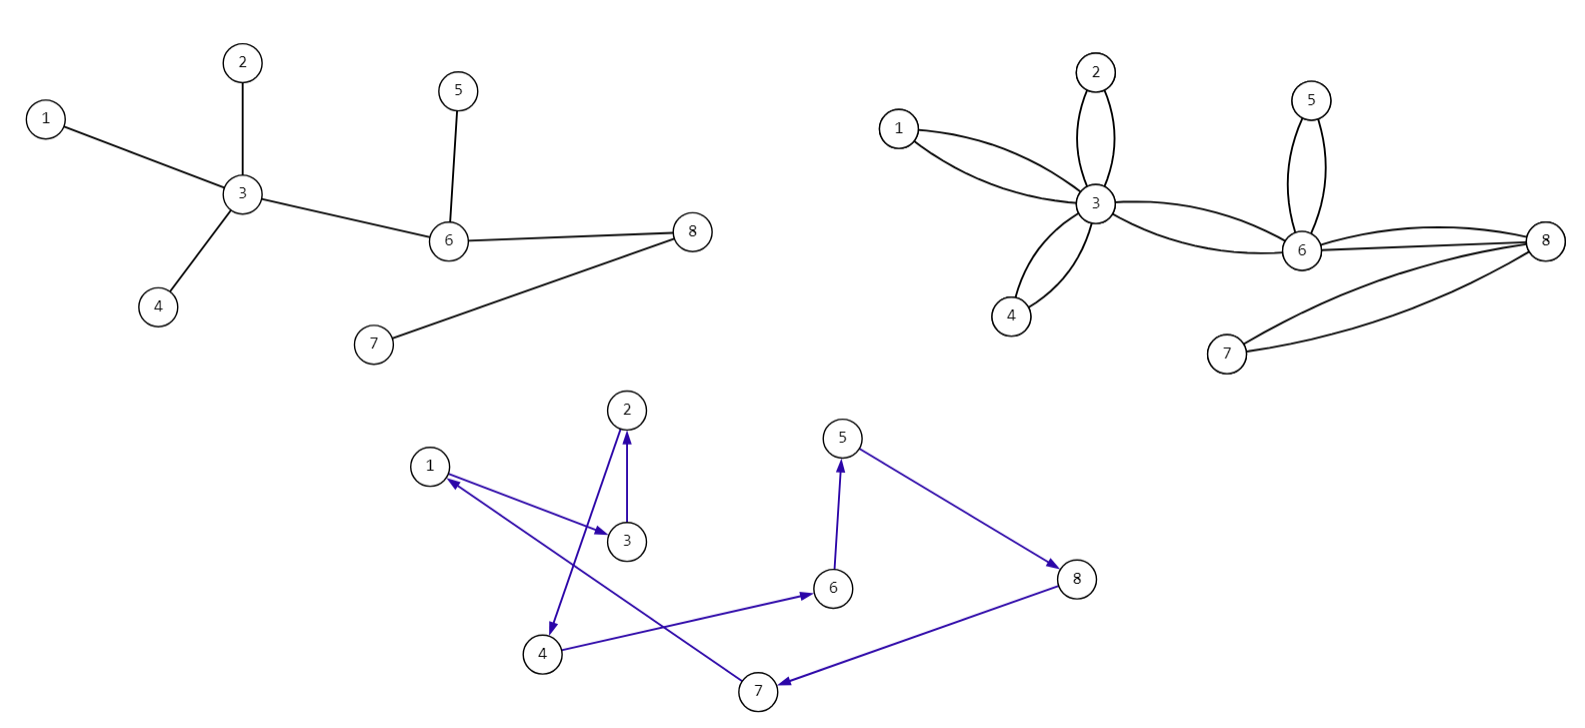
\includegraphics[width=17cm]{img/pic1_algo.png}
    \centering
\end{figure}

\subsubsection{Корректность}
\begin{proposition}
    Пусть $H$ - гамильтонов цикл и $T$ - MST. Тогда $w(H) \geq w(T)$, где $w$~-- сумма весов ребер.
\end{proposition}
\begin{proof}
    Если убрать 1 ребро из гамильтонова цикла получим дерево, вес которого не меньше веса \textsf{MST} по определению.
\end{proof}

\begin{proposition}
    Алгоритм~\ref{alg:two} дает 2-приближение МЗК.
\end{proposition}

\begin{proof}
    Пусть \textsf{OPT} это истинное решение МЗК -- гамильтонов цикл. Тогда по предыдущему утверждению, $2 \cdot w($\textsf{OPT}$) \geq 2 \cdot w($\textsf{T}$) = w(\tau)$. 
    Но мы обходим граф не по ребрам, а сразу напрямую от вершины к вершине. Очевидно, наша оценка не ухудшиться по неравенству треугольника.
\end{proof}

\subsubsection{Асимптотика}
\begin{proposition}
    Алгоритм~\ref{alg:two} работает за $\mathcal{O}(n^2)$.
\end{proposition}

\begin{proof}
    \textsf{MST} строится алгоритмом Прима за $\mathcal{O}(m + n\log{n})$. Поиск эйлерова цикла и обходы графов, в том числе добавление ребер, работает за линию от числа вершин. Но так как мы работаем в метрическом пространстве, то ребер всего $n^2$.
\end{proof}

\subsection{Алгоритм $\frac{3}{2}$-приближения}
В первом алгоритме мы искали эйлеров цикл и обходили его, но что если существует эйлеров цикл весом меньше? Мы знаем, что эйлеров цикл существует $\Leftrightarrow$ если все вершины четной степени. Улучшим наш алгоритм, используя эти знания.

\begin{definition}
    Совершенным паросочетанием называется паросочетание, которое включает все вершины.
    То есть любая вершина инцидента какому-либо ребру из паросочетания.
\end{definition}

\subsubsection{Описание}
\RestyleAlgo{ruled}
\begin{algorithm}
\caption{Алгоритм  $\frac{3}{2}$-приближения МЗК}\label{alg:twothree}
1. Пусть $T =$ \textsf{MST}($G$). \\
2. Выделим вершины $ODD$ с нечетными степенями из $T$ и построим совершенное паросочетание $M$ минимального веса на $G\vert_ODD$. \\
3. Добавим ребра из паросочетания в $T$ и строим эйлеров цикл $\tau$ на нем. \\
4. В любом порядке обойти цикл и вывести первые вхождения вершин.
\end{algorithm}

\begin{figure}[!h]
    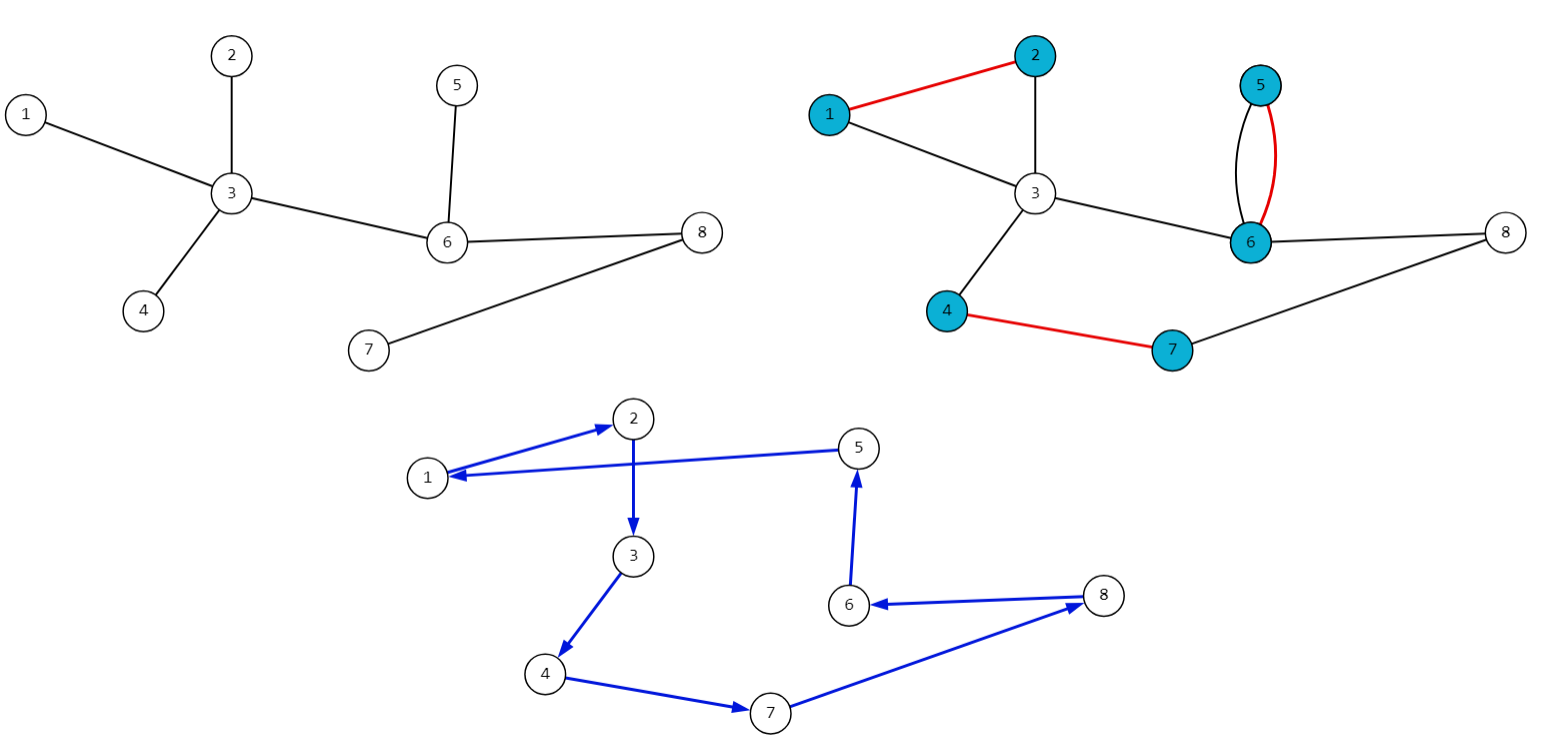
\includegraphics[width=17cm]{img/pic2_algo.png}
    \centering
\end{figure}

\subsubsection{Корректность}
\begin{proposition}
    Для вершин $T$ нечетных степеней существует совершенное паросочетание. 
\end{proposition}
\begin{proof}
    $\sum^{n}_{i=1}deg(v_i) = 2|E|$. Отнимем вершины четных степеней и получим опять же четное число, то есть нечетных вершин всегда четное количество.
\end{proof}

\begin{proposition}
    Пусть $V' \subset V$ такой, что $|V'|$ четно, и пусть $M$ совершенное паросочетание минимального веса на $V'$. Тогда, $w(M) \leq \textsf{OPT}/2$.
\end{proposition}
\begin{proof}
    Пусть существует решение МЗК -- обход $\tau$, где $w(\tau) = \textsf{OPT}$. Ограничим наш обход вершинами из $V'$, то есть $\tau' = \tau\vert_{V'}$. Снова получим какой-то обход, где $w(\tau') \leq w(\tau)$ по неравенству треугольника. Заметим, что обход $\tau'$ это объединение двух совершенных паросочетаний, ребра которых чередуются в цикле. Из этого факта и из того, что $M$ совершенное паросочетание минимального веса следует, что $w(M) \leq w(\tau') / 2 \leq w(\tau) / 2 =  \textsf{OPT} / 2$.  
\end{proof}
\begin{proposition}
    Алгоритм~\ref{alg:twothree} дает $\frac{3}{2}$-приближение МЗК.
\end{proposition}

\begin{proof}
    Пусть $\tau$ - наш эйлеров цикл из алгоритма, $ans$ - вывод алгоритма. Тогда выполняется цепочка неравенств:
    $$w(ans) \leq w(\tau) = w(T) + w(M) \leq \textsf{OPT} + \textsf{OPT} / 2 = \frac{3}{2}  \textsf{OPT}$$
\end{proof}

\subsubsection{Асимптотика}
\begin{proposition}
    Алгоритм~\ref{alg:twothree} работает за $\mathcal{O}(n^4)$.
\end{proposition}

\begin{proof}
    Имеем то же слагаемое в виде $\mathcal{O}(n^2)$ из Алгоритма~\ref{alg:twothree}, но теперь нам нужно найти совершенное паросочетание минимального веса. Для этого можно использовать комбинаторный алгоритм\hyperref[litlink2]{$^{[2]}$}, который использует невзвешенный алгоритм Эдмондса в качестве подпрограммы за $\mathcal{O}(n^2m)$, где $m = \mathcal{O}(n^2)$ для полного графа.
\end{proof}
\newpage
\subsubsection{Анализ работы алгоритма}
Будем генерировать точки на плоскости в пределах прямоугольника от $\left(0, 0\right)$ до $\left(100, 100\right)$. Напишем два генератора, один из которых кидает точку равномерно, а другой генерирует несколько кластеров точек с помощью гауссовских векторов. 

Попробуем сначала оценить точность случайных тестах --- на равномерных и гауссовских векторах. Будем тестировать при малых $n$ чтобы мы нашли точное решение перебором за адекватное время.

\begin{figure}[h!]
    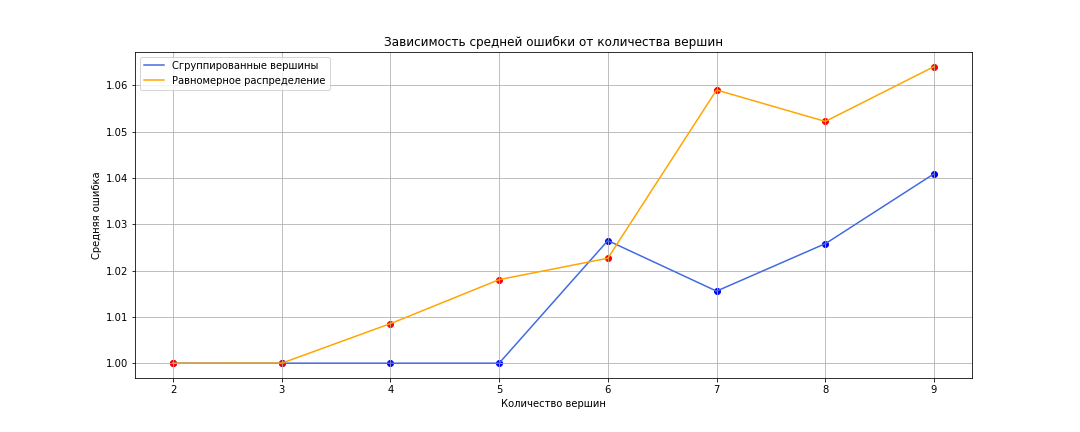
\includegraphics[width=18cm]{img/graph3.png}
    \centering
    \caption{Точности алгоритмов.}
\end{figure}

Заметим, что на сгруппированных вершинах наш алгоритм приближает точнее чем на равномерно раскиданных точек. Это логично, так как чем ближе находятся точки, тем меньше ошибка. Интуитивно, можно просто сжимать вершины принадлежащие одному кластеру.

\newpage

Теперь рассмотрим время работы для больших $n$. Уже можно не запускать переборный алгоритм, так как мы уже не считаем ошибку. Запустим сначала на равномерно распределенных вершинах.

\begin{figure}[h!]
    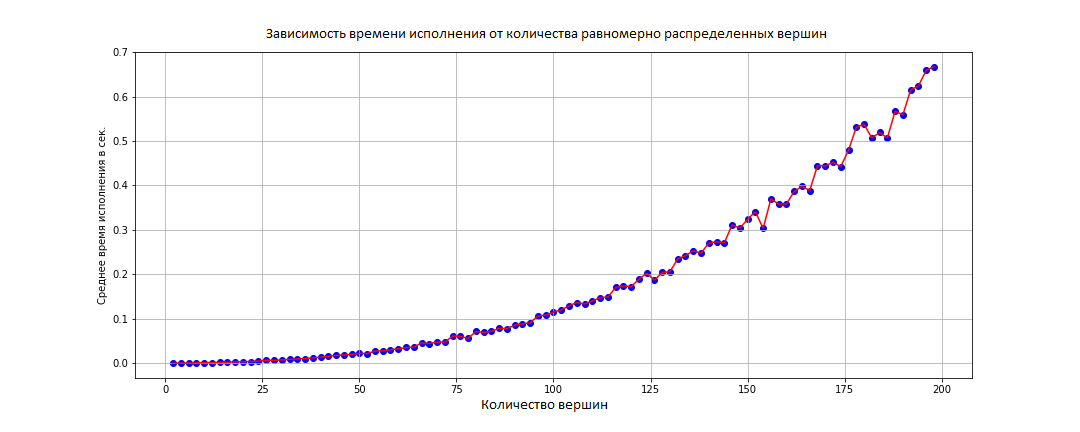
\includegraphics[width=18cm]{img/graph0.png}
    \centering
    \caption{Время работы для случайных вершин.}
\end{figure}

Но интереснее будет посмотреть на зависимость времени работы от количества кластеров.

\begin{figure}[h!]
    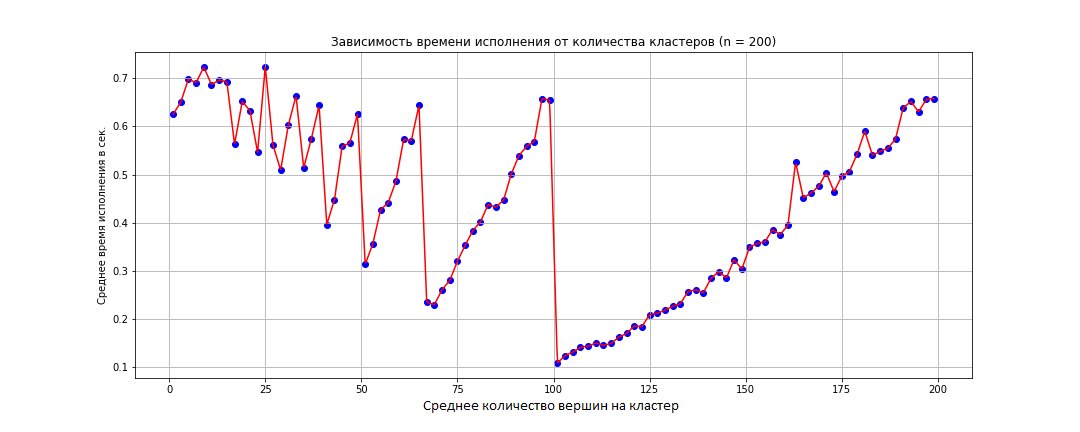
\includegraphics[width=18cm]{img/graph_gauss.png}
    \centering
    \caption{Время работы для сгруппированных вершин.}
\end{figure}

На этих тестах количество кластеров выбирался как $\lfloor n / k \rfloor$, где $k$ -- среднее количество вершин на кластер. Не трудно заметить, что скачок вниз происходит тогда, когда $k$ делит $n = 200$ примерно нацело. Это означает, что количество кластеров увеличивается.


Получается, что наш алгоритм очень хорошо работает для кластеризованных графов~--- когда вершины неявно скучкованы.

\subsubsection{Достижимость верхней оценки}

Рассмотрим граф из треугольников как на рисунке 4 когда $n$ - нечетное. Пусть \textsf{MST} стала центральная кривая, которая идет по зигзагу. Тогда всего 2 вершины (конечные) будут иметь нечетную степень. В итоге имеем цикл длиной $(n + 1) + \lfloor n / 2 \rfloor$.
\begin{figure}[h!]
    \centering
    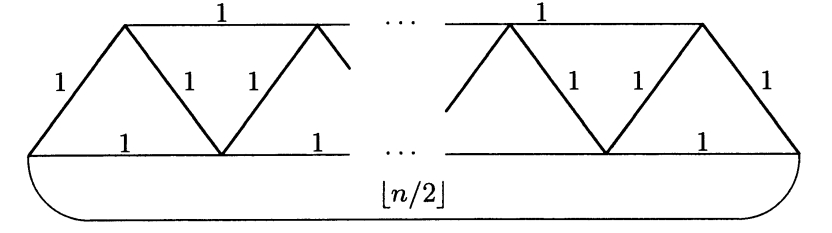
\includegraphics[width=17cm]{img/sample.jpg.png}
    \caption{Граф для верхней оценки.}
\end{figure}


\section{Выводы}
Мы рассмотрели два полиномиальных алгоритма, которые неплохо приближают решение метрической задачи коммивояжёра. Они довольно простые, но работают на разных графах по разному. Все эффективные (сокращающие полный перебор) методы решения задачи коммивояжёра — методы эвристические. Большинство эвристических методов находит не самый эффективный маршрут, а приближённое решение. Я считаю, что $\frac{3}{2}$ уже отличный результат для таких сложных задач.

\newpage
\section{Приложение}

\begin{figure}[h!]
    \centering
    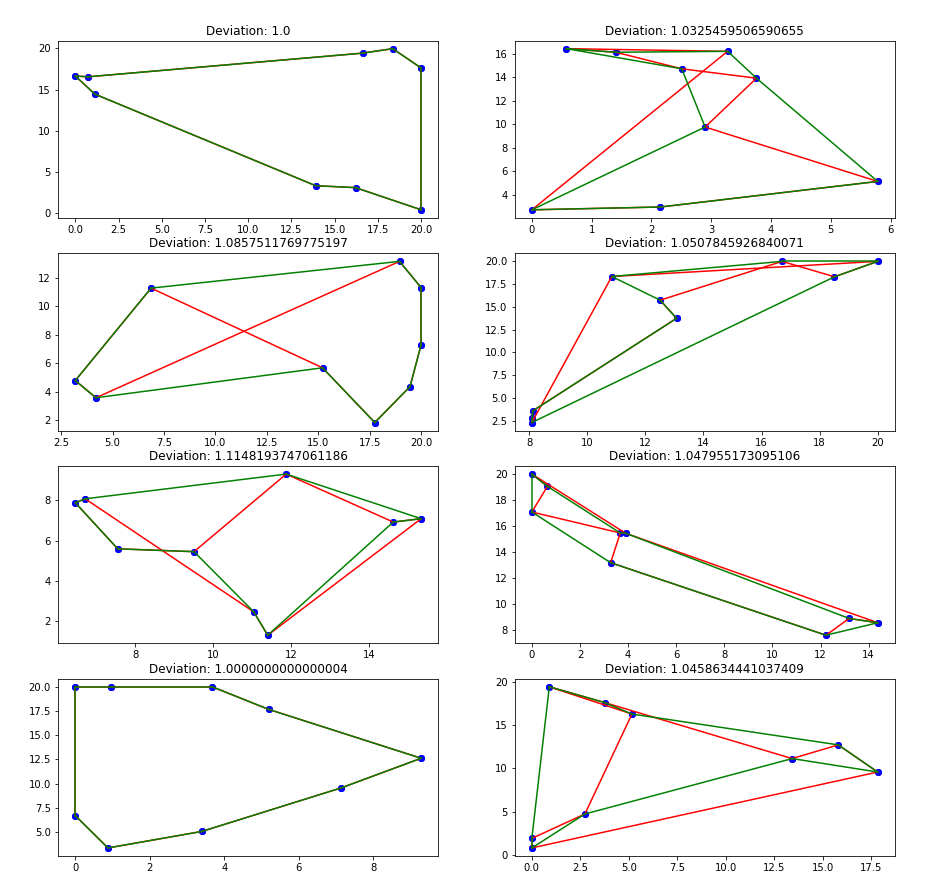
\includegraphics[width=18cm]{img/samples_gauss_fixed.png}
    \caption{Несколько примеров работы алгоритма.}
\end{figure}

\addcontentsline{toc}{section}{Список литературы}

\begin{thebibliography}{}
    \bibitem{litlink1} Vazirani, V. Approximation Algorithms, Springer, 2001.

    \bibitem{litlink2} Kolmogorov, Blossom V: A new implementation of a minimum cost perfect matching algorithm. \url{https://pub.ista.ac.at/~vnk/papers/BLOSSOM5.html}
\end{thebibliography}



\end{document}
